\documentclass[a4paper,10pt]{article}
\usepackage[margin=2cm]{geometry}

%%% Language and encoding %%%
\usepackage[utf8]{inputenc}
\usepackage[T1]{fontenc}
%%% Mathematical symbols and notations %%%
\usepackage{amsthm, amsmath, mathrsfs, amssymb}
\usepackage{textcomp}
\usepackage{algorithm}
\usepackage{algorithmic}

%%% Figures %%%
\usepackage{caption, subcaption}
\usepackage{tikz}
\usepackage{tkz-graph}
\usetikzlibrary{shapes, shapes.gates.logic.US, trees, positioning, arrows, decorations.pathreplacing, plotmarks, backgrounds,shapes}
%%% Other packages %%%
\usepackage[affil-it]{authblk}
\usepackage{multirow}
\usepackage{xcolor}
\definecolor{bleuclairimtatlantique}{RGB}{0,184,222}
\definecolor{noirimtatlantique}{RGB}{60, 60, 60}
\definecolor{blancimtatlantique}{RGB}{255, 255, 255}
\definecolor{bleufonceimtatlantique}{RGB}{12, 35, 64}
\definecolor{vertimtatlantique}{RGB}{164, 210, 51}
\definecolor{grisimtatlantique}{RGB}{230, 230, 230}
\definecolor{ocre}{RGB}{250,82,20}
\usepackage{url}
\usepackage{hyperref}
\usepackage{verbatim}
\usepackage{varwidth}
%% Define the figures path
\newcommand{\inputfig}[1]{\input{figures/#1}}
\graphicspath{{figures/}}

%\usepackage{empheq}
\usepackage[framemethod=tikz]{mdframed}

%%%%% Definition of commands %%%%%
\newcommand{\loc}{\mathcal{L}}
\newcommand{\cu}{\mathcal{C}}
\newcommand{\su}{\mathcal{S}}
\newcommand{\ro}{\mathcal{R}}

%%%%% Definitions for tikz %%%%%
% Definition of styles for diagrams :
\tikzset{%
    % Symbols for block diagrams
    block/.style    = {draw, thick, rectangle, minimum height = 3em,
    minimum width = 3em},
    sum/.style      = {draw, circle, node distance = 2cm}, % Adder
    input/.style    = {coordinate}, % Input
    output/.style   = {coordinate}, % Output
    % Gates and symbols style for the fault trees
    and/.style={and gate US,thick,draw,fill=red!20,rotate=90,
    anchor=east,xshift=-1mm},
    or/.style={or gate US,thick,draw,fill=blue!20,rotate=90,
    anchor=east,xshift=-1mm},
    be/.style={circle,thick,draw,fill=green!20,anchor=north,
    minimum width=0.7cm},
    tr/.style={buffer gate US,thick,draw,fill=purple!40,rotate=90,
    anchor=east,minimum width=0.8cm},
    % Label style
    label distance=3mm,
    every label/.style={blue},
    % Event style
    event/.style={rectangle,thick,draw,fill=yellow!10,text width=2cm,
    text centered,font=\sffamily,anchor=north},
    % Children and edges style
    edge from parent/.style={very thick,draw=black!70},
    edge from parent path={(\tikzparentnode.south) -- ++(0,-1.05cm)
    -| (\tikzchildnode.north)},
    level 1/.style={sibling distance=7cm,level distance=1.4cm,
    growth parent anchor=south,nodes=event},
    level 2/.style={sibling distance=7cm},
    level 3/.style={sibling distance=6cm},
    level 4/.style={sibling distance=3cm},
    %%  For compatability with PGF CVS add the absolute option:
    absolute
}

\tikzstyle{client}=[regular polygon,regular polygon sides=3,draw,fill=blue!50,fill opacity=1,scale=0.4]
\tikzstyle{ptf}=[draw,circle,fill=red!50,fill opacity=1,scale=0.8]
\tikzstyle{cdc}=[regular polygon, regular polygon sides=3,draw,fill=yellow!70,fill opacity=1,scale=1.2]

\tikzstyle{legend}=[scale=0.7,right,text justified]
\tikzstyle{shipment}=[->,>=stealth',blue]
\tikzstyle{ftlarc}=[->,>=stealth',very thick,red]
\tikzstyle{vertexD}	=[circle,draw=black!80,fill=purple!70,minimum size=7pt,inner sep=0pt]
\tikzstyle{vertex0}	=[circle,draw=black!80,fill=purple!20,minimum size=7pt,inner sep=0pt]
\tikzstyle{j0}			=[circle, draw=black,fill=purple,minimum size=13pt,inner sep=0pt, scale=1]
\tikzstyle{farm}		=[circle, draw=black,fill=blue!80,minimum size=4pt,inner sep=0pt, scale=1]

\tikzstyle{com2}		= [minimum size=0pt,inner sep=0pt, scale=1]
\tikzstyle{edgetr} 	= [draw,thick,->,purple]
\tikzstyle{edge1} 	= [draw,dotted,-,blue, thick]



\title{Location Inventory Routing Problem: new formulation and sampling heuristic}
	
\author{Guillaume Massonnet$^{1,2}$, Olivier P\'eton$^{1,2}$}
	
\date{$^1$ IMT Atlantique\\ 
	$^2$ LS2N UMR CNRS 6004 (Laboratoire des Sciences du Numérique de Nantes), \\ 4 rue Alfred Kastler, F-44307 Nantes Cedex, France}
	%\cortext[cor]{Corresponding author. name address}
	


\begin{document}
	
\maketitle


\begin{abstract}
	blablabla
	
	
\textbf{Keywords:}		location, inventory management, routing, sampling heuristics, supply chain
	
\end{abstract}




\modulolinenumbers[5]
\linenumbers
\begin{linenumbers}


\section{Introduction}

For any business, the stock is a major financial asset. 
Therefore, its volume must be controlled in order to avoid stock-out and minimize holding costs. 
The Vendor managed inventory (VMI) is based on the principle that the company selling a product has only a stock directly dedicated to the delivery to customers. In other words, all items received are placed on the shelf and stock replenishment is the responsibility of the supplier. VMI had motivated much research about the joint optimization of the inventory and transport, leading to the inventory routing problem (IRP). The IRP considers one supplier running a fleet of vehicles and a set of customers who consume a good on a multi-period time horizon. The objective of the IRP is to jointly optimize the delivery schedule of customers, the quantities delivered, and the delivery routes to be covered in each period, while minimizing the sum of routing costs and storage costs.

Traditional applications of the IRP have been listed in the survey \cite{Coelho2014}. They mainly concern the distribution of commodities, raw materials or fast moving consumer goods. These activities rely on a stable supply chain network. 
In industrial applications the set of customers is quite stable and the starting points of all defined for a long duration.
For example, distribution of fuel always starts from the same fuel depots, which capacity and location cannot be easily modified. 

In this paper we consider an extension of the IRP concerning emerging activities which supply chain is not yet designed, 
or any activity has to frequently revise its supply chain design, e.g. delivery of e-commerce goods or services to a set of customers that changes over time. We assume a three-level supply chain consisting of one production facility, several intermediate depot called distribution centers (DC) and a larger set of customers. A single product is first carried from the production facility to DCs, and then from DCs to customers. The decision variables concern the location of DCs, the allocation of customers to DC and all IRP decisions previously cited. 
This optimization problem is called the Location Inventory Routing Problem (LIRP). This problem appeared recently in the scientific literature \citep{AhmadiJavid2010} and has been more and more studied since then. 

The contributions of this paper are the following. 
In section \ref{sec:lit}, we review the scientific literature dedicated to the LIRP. 
In section \ref{sec:model}, we propose a new mathematical formulation of the LIRP and show that this formulation is general enough to 
cover several types of supply chain networks. 
In section \ref{sec:algo}, we propose a matheuristic algorithm based on the iterative sampling of the routes. 
In section \ref{sec:expe}, we introduce new LIRP instances and report numerical expriment that show the performance of our algorithm.

\section{Literature Review} \label{sec:lit}



\subsubsection*{Generalites sur les problèmes combines}

The LIRP combines three families of well-known optimization problems: vehicle routing, facility location and inventory management. 
As shown in Figure \ref{fig:circles}, these problems, combined in pairs, already define the location routing problem (LRP), the inventory routing problem (IRP) and the location problem with inventory management (ILP). 

   	\begin{figure}[htbp]
	\centering
	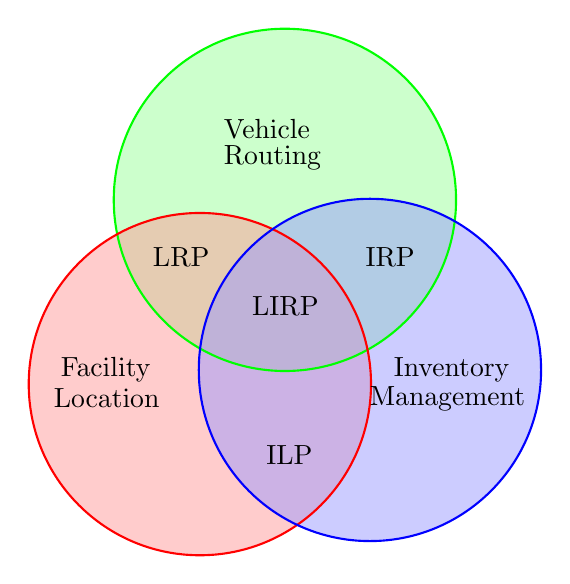
\begin{tikzpicture}[scale=0.18, auto,swap]
	\coordinate (A) at (0,1);
	\coordinate (B) at (12,2);
	\coordinate (C) at (6,14);
	\fill[opacity=0.5,green!40] (C) circle(12);
	\fill[opacity=0.5,red!40] (A)  circle(12);
	\fill[opacity=0.5,blue!40] (B)  circle(12);
	\fill[green,even odd rule] (C) circle(12) circle(12.15);
	\fill[red,even odd rule] (A) circle(12) circle(12.15);
	\fill[blue,even odd rule] (B) circle(12) circle(12.15);
	
	\draw (-10.5,2) node[right] {Facility};
	\draw (-11,0) node[right] {Location};
	\draw (13,2) node[right] {Inventory};
	\draw (11.3,0) node[right] {Management};
	\draw (1,19) node[right] {Vehicle};
	\draw (1,17) node[right] {Routing};
	\draw (4,-4) node[right] {ILP};
	\draw (3,6.5) node[right] {LIRP};
	\draw (-4,10) node[right] {LRP};
	\draw (11,10) node[right] {IRP};
	\end{tikzpicture}
	\caption{Optimization problems combining facility location, inventory management and routing}
	\label{fig:circles}
	\end{figure} 

These three integrated problems have already been the subject of many publications in recent decades.

\begin{itemize}
	
	\item \textbf{IRP: }
	
	The inventory problem has been studied for more than 30 years \citep{Coelho2014}. Prior surveys had been published by \cite{Campbell98}, \cite{MoinSalhi2007}. Interested reader may also read the tutorial by \cite{Bertazzi2012}. 
	
	Very few models consider the inventory routing problem within a two-echelon or multi-echelon network	\citep{GuimaraesCoelho2019}
	
	\item \textbf{LRP: }
	
	The Location Routing problem has been introduced 
	
		
	
	\cite{Laporte1987} 
	
	Surveys by \cite{MinJS98}, \cite{NagySahli07}, \cite{ProdhonPrins2014}, \cite{DrexlSchneider2015} and \cite{Schneider2017} 
	
	
	
In the context of arc routing, 	\cite{Riquelme2016} inr

	
	
	\item \textbf{ILP : }
	
	As pointed by \cite{Melo2009}, facility location is frequently combined with inventory decisions. However, the integration of inventory and location decisions in a single mathematical model did not give rise to a well-identified optimization problem such as IRP or LRP. 
	
	
\end{itemize}

\subsection{Review of the literature}

The location inventory routing problem LIRP has been attracting much research effort in the very recent years, but preliminary works have appeared several decades ago.  
In this section, we review the main publications related to the LIRP.
Section \ref{sec:almost} summarizes the preliminary works that led to a formal definition of the LIRP. 
Next sections described the modeling of the main LIRP components: location and supply chain desgin (section\ref{sec:l}), 
routing (\ref{sec:r} and inventory policies (\ref{sec:i}). 

\subsection{Preliminary works related to the LIRP}
\label{sec:almost}

 The idea of integrating location, inventory and routing decisions in mathematical models is not new, but most models have been considered intractable until the recent progress of mathematical programming solvers and heuristic solution methods. 
In 1988, \cite{PerSir88} pointed the necessary interdependance between location, inventory and routing decisions. 
The authors proposed an integrated model combining location and inventory decisions, but only direct shipments were considered and no computational experiments were presented. 
This model has been extended by \cite{AmbScu05} to a multi-level problem with distribution routes visiting several customers. The authors also propose a dynamic models (with multiple periods). Computational experiments show the practical difficulty of solving static models (with one time period). 

\cite{DasCShen02} study a joint location-inventory model with risk pooling, facility location, vehicle routing, and inventory control.

Several LIRP related papers considered the three main decisions in a hierarchical way, or priority is given to one or two decisions. 
In \cite{LiuLee03} and \cite{LiuLin05}, inventory mangement decisions are taken independently from routing and location. 
\cite{Shen07} explicitly model facility location and allocation decisions but use approximated routing costs instead of formal routing costs. 
\cite{MetZab10} propose a two-stage stochastic programming approach for a medical supply
storage and distribution problem.
At the first stage, storage locations and the optimal inventory policy are determined. 
At the second stage, a recourse routing plan is optimized for each disaster scenario. 
Routing decision are decoupled from location and inventory decisions. 
Hence, all these references cannot be \textit{stricto sensu} considered as LIRP models. 

\subsection{Supply chain design}
\label{sec:l} 

As an integrated optimization problem, the LIRP usually arises in complex logistics networks with several layers of facilities. 
Depending on the volume of the shipments, transport can be organized in full truckload (FTL) or less than truckload (LTL) legs. 
In FTL transport, shipments are sent directly from their origin to their destination. In LTL transport, routes have one origin and several delivery points. The roads are therefore multi-clients. The presence of a ``routing'' component in the LIRP assumes the existence of routes visiting multiple sites, at least in one part of the supply chain.
The vast majority of LIRP articles deal with three-layer networks such as that illustrated in Figure \ref{fig:directloop}. 
Direct routes are performed between a production facility (large red circle) delivers a set of depots or distribution centers (small red circles). A second echelon includes routes visiting several end customers (blue circles).

\begin{figure}[htbp]
	\centering
	\inputfig{model1}
	\caption{LIRP model with direct+route supply chain design}
		\label{fig:directloop}
	\end{figure}

Several papers deviate from this main scheme.  \cite{Zhang2014} consider only 2 layers: a set of candidate depots and customers. Routes start at a depot and visit several customers ; no inventory decision is made at depots. 

\cite{AmbScu05} and \cite{Tavana2018} extend the main logistics scheme to a 4 layer network. Shipments are direct in the upper echelon whereas LTL routes are performed in the two lower echelons. 
\cite{Eskandari2018} study a blood supply chain with 4 layers. They consider direct shipment between the first three layers and multi-point routes for the final delivery. 
\cite{Bashiri2018} consider a network with multi-point routes at the first echelon and direct deliveries at the second echelon. 
Finally, \cite{Riquelme2016} introduce the location arc routing problem with inventory constraints. 

Moreover, only a few papers (\cite{LiuChenLiLiu2015}, \cite{Deng2016}, \cite{Zhalechian2016} and \cite{LiGuoWangFu2013} 
consider a closed-loop supply chain. 


\subsection{Route formulation}
\label{sec:r}

A large majority of the LIRP mathematical models uses an arc-based representation of the routes. 
However, in many applications, the number of customer visited within a route is limited by a number of practical constraints (time constraints, stopover costs, detour constraints). \cite{MaDav05} propose a distribution chain design  minimizing location fixed costs, inventory costs and transportation costs. They observe that vehicles can only serve one site in their journey, and thus, do not model a full LIRP model. 

\cite{Guerrero2013} propose a route-based model with an exponential number of routes. A relaxation of the model is decomposed into an inventory location problem and a routing problem which is solved by column generation. 
The model in \cite{Lehrlaly2016} is based on all feasible routes with no more than three customers. 
Route based models are also used in \cite{LiGuoWangFu2013}, \cite{LiuChenLiLiu2015},  \cite{Deng2016} and \cite{hiassat_genetic_2017} 
but these papers do not detail routes generation.

\subsection{Inventory policies}
\label{sec:i}

As far as inventory management is concerned, the literature can be classified in two main families: papers considering a continuous time inventory policy 
and those who consider discretized time periods. 
In the first case, demand is considered either constant (see e.g. \cite{AhmSed2012}, \cite{Deng2016}) or subject to a known distribution a 
normal distribution (see e.g. \cite{Nekooghadirli2014}, \cite{Zhalechian2016}, \cite{Saragih2018}) or a Poisson distribution (see e.g. \cite{Asadi2018}, \cite{HabibiAS2018}). In these cases, classical continuous review policies such as $(r,Q)$ and $(S-1,S)$ policies are applied \textcolor{red}{Guillaume, il faut qu'on discute de ça} and the same inventory cycle repeats over time. Note that in this category, the objective function often incorporate the average value of inventories or their standard deviation, which yield non linearity. Thus, only small instances can be solved by MINLP solvers, or general purpose heuristics and metaheuristics are used. 


In the latter category, the time horizon is decomposed into several time periods and all demands and flow values within one period are aggregated. This leads to inventory management policies that look like lot-sizing policies. Most references study models in which all data including demand are variable but deterministic (see e.g. \cite{Guerrero2013}, \cite{Zhang2014}, \cite{Ghorbani2016}). 
\cite{Vahdani2018} consider stochastic storage capacity. 
\cite{Rayat2017} explicitly model stochastic demand and propose an MINLP bi-objective model with multiple periods and multiple products. The model is solved with an epsilon constraint and several multi-objective metaheuristics. 
Uncertainty can also be incorporated through various modeling techniques. 
\cite{ChenChenSunLiu2014, TavakkoliIFAC2016} model fuzzy demand ; \cite{Bashiri2018} define demand scenarios ; 


Tables \ref{tab1} and \ref{tab2} present a synthesis of the main bibliographic references concerning the LIRP. 
Tables \ref{tab1} presents models with continuous time inventory policies. 


\textcolor{red}{Ajouter texte pour presenter le contenu de chaque colonne}

\begin{table}[htbp]
	\scriptsize
\begin{tabular}{lccccccc}
	\toprule
	Reference & Periods & Route & Layers   & Flow &  Stochastic & Linear & Inventory \\
             &          & model & 		   & 	   &     demand        &        & policy                 \\
 \midrule
\cite{Yuchi2016}	&	1	&	arc	&	3 &	direct+loop	&	constant	&	NL	&	Wilson	\\	
\cite{AhmadiJavid2010}	&	1	&	arc  &	3 &	direct+loop	&	normal	&	NL	&	(r,Q) 	\\	
\cite{AhmSed2012}	&	1	&	arc &	3 	&	direct+loop	&	constant 	&	NL	&	(0,Q)	\\	
\cite{Nekooghadirli2014}	&	multi	&	arc &	3 	&	direct+loop	&	normal 	&	NL	&	(r,Q) 	\\	
\cite{Seyedhosseini2014} &	1	&	arc	&3 &	direct+loop	&	demand	&	NL	&	(r,Q) 	\\	
\cite{LiuChenLiLiu2015}	&	1	&	route	&	3 	&	direct+loop	&	normal	&	NL	&	(r,Q) 	\\	
\cite{Tang2016}	&	1	&	arc	&	3 	&	direct+loop	&	no	&	NL	&	(Q, R)	\\	
\cite{Zhalechian2016}	&	multi	&	arc	&	3 	&	direct+loop	&	Normal	&	NL	&	(r,Q) 	\\	
\cite{Deng2016} & 1	&	route	&	3 	&	direct+loop	&	no	&	NL	&	(r,Q) 	\\	
\cite{Dehghani2017}	&	1	&	arc	&	3 	&	direct+loop	&	Poisson	&	NL	&	(S-1,S)	\\	
\cite{Rafie-Majd2018}	&multi	&	arc	&	3 	&	direct+loop	&	normal	&	NL	&	(Q,R)	\\	
\cite{HabibiAS2018}		&	1	&	arc	&	3 &	direct+loop	&	 Poisson 	&	NL	&	(S-1,S)	\\	
\cite{Asadi2018}		&	1	&	arc	&	3 	&	direct+loop	&	Poisson 	&	NL	&	(S-1,S)	\\	
\cite{Saragih2018}	&	1	&	arc	&	3 	&	direct+loop	&	 normal	&	NL	&	(r,Q) 	\\	
\cite{Sajjadi2011}	&	1	&	arc  	&	3	&	direct+loop	&	yes	&	NL	&	fixed interval \\	
\cite{ChenChenSunLiu2014}	&	1	&	arc	&	3 	&	direct+loop	&	fuzzy 	&	L	&	Periodic (T,$r_j$)	\\	
\cite{Zheng2019}		&   1		& arc		& 2		& loop					&  demand (avg,std) & NL & Periodic review \\
\bottomrule
\end{tabular}
\caption{Reference with continuous inventory review}
	\label{tab1}
\end{table}

Table \ref{tab2} presents models with time discretization. 

\begin{table}[htbp]
	\scriptsize
	\begin{tabular}{lcccccc}
		\toprule
		Reference & Periods & Route & Layers   & Flow &  Stochastic & Linear  \\
					&          & model & 	   & 	   &     demand        &                      \\
		\midrule
\cite{AmbScu05}			&	1 \& multi	&	arc		&	4 	&	direct+loop+loop	&	no	&	L		\\
\cite{Zhang2014}		&	multi		&	arc  	&	2 	&	loop				&	no	&	L	\\
\cite{Guerrero2013}		&	multi		&	route	&	3 	&	direct+loop			&	no	&	L	\\
\cite{TavakkoliIFAC2016}&	multi		&	arc		&	3 	&	direct+loop			&	fuzzy 	&	L	\\
\cite{Ghorbani2016}		&	multi		&	arc		&	3 	&	direct+loop			&	no	&	L\\
\cite{Lehrlaly2016}		&	multi		&	route	&	3 	&	direct+loop			&	no	&	L		\\
\cite{Rayat2017}		&	multi		&	arc		&	3 	&	direct+loop			&	demand (avg, std)	&	NL		\\
\cite{Hiassat2017}		&	multi		&	route	&	3 	&	direct+loop			&	no	&	L		\\
\cite{Riquelme2016}		&	multi		&	arc		&	2 	&	general graph		&	no	&	L	\\
\cite{Tavana2018} 		&	multi		&	arc		&	4 	&	direct+loop+loop 	&	no	&	L		\\
\cite{Vahdani2018}		&	multi		&	arc		&	3 	&	direct+loop			&	storage capacity	&	L	\\
\cite{Eskandari2018}	&	multi		&	arc		&	4 	&	direct+direct+route	&	yes (disaster)	&	L		\\
\cite{Bashiri2018}		&	multi		&	arc		&	3 	&	loop+direct			&	demand (scenarios)	&	L	\\
		\bottomrule
	\end{tabular}
	\caption{Reference with time discretization}
	\label{tab2}
\end{table}




\subsection{Contribution of this paper}

This paper brings contribution in the LIRP literature in three ways. First, we propose new route-based mathematical model that covers both FTL and LTL routes between any layer of the logistics network. Without loss of generality we present this model on a three layer supply chain with one production facility, a set of candidate distribution centers and a larger set of customers. 
Second, we propose a sampling solution method based on the decomposition of large instances in several smaller instances that are tractable by an MILP solver. 
Finally, we introduce new instances for the LIRP and present computational experiments that show the relevance of our approach. 


\newpage

\section{Mathematical model}

\label{sec:model}

\subsection{Problem settings and notations}
%\begin{table}[htbp]
%	\centering
%	\begin{tabular}{ll}
%		\toprule
%		$\kd$ & Capacity of vehicles delivering distribution centers\\ 
%		$\kc$ & Capacity of vehicles delivering customers\\ 
%		$\nu_{\dc}$ & fleet size for vehicles delivering distribution centers\\ 
%		$\nu_{\cu}$ & fleet size for vehicles delivering customers\\ 
%		$\alpha_{ir}$ & indicator of route $r\in\rc$ visits customer $i$\\
%			\bottomrule
%		
%	\end{tabular}
%	\caption{Reste à définir}
%	\label{tab:set}
%\end{table}



We consider a two echelon distribution network composed of one production facility, a set of customers and a set intermediate logistics facilities called distribution centers (DC). 
The list of customers as well as their demand are assumed deterministic for a given time horizon $T$, typically a few weeks. 
The set of customers is denoted by $\cu$ and the demand of customer $i \in \cu$ at time period $t\in T$ is denoted by $d^t_i$.
The set of potential DCs on a level $k$ denoted by $\loc_k$.
Selecting a DC incurs a fixed opening cost $f_j$ for each DC. This cost is paid once at the beginning of the planning horizon. 
Note that the choice of selected DCs cannot be modified during the whole period. 

Goods can be delivered to a DC before they are sent to customers. In the same ways, goods can be delivered to customers before they are actually used by customers. In theses cases a holding cost $h^t_i$ is payed for every good stored at facility $i \in \loc$ at period $t$.
The initial inventory at facility $i \in \loc$ is denoted by $I_i^0$. 
We assume that the amount of inventory stored at facility $i \in \loc$ cannot excess a maximal value $I_i^{\max}$. 

As far as routing is concerned, we propose a unified model that covers a broad spectrum of potential applications and distribution modes (FTL, LTL). 
Our model is based on a set of existing routes at each echelon. 
This set can be large but enumerable. 
Route at level $k$ are denoted by $\ro_k$. 
They start from the production facility and visit one or several DCs before returning to the production facility. 
For any route $r \in \ro$, the indicator $\gamma_{jr}$ has value 1 is $r$ visits DC $j \in \loc\setminus{\cu}$, and 0 otherwise. 
Similarly, delivery routes $\ro_L$ at the lower echelon start from a DC, visit one or several customers and return to the same DC. 
For any route $r \in \ro_L$, the indicator $\alpha_{ir}$ has value 1 is $r$ visits customer $i \in \cu$, and 0 otherwise. 

Each route 	$r\in \ro$ has a fixed cost 	$c_r$ which is independent of the load carried. 

%% ICI %%%



Using a route to deliver units during a time period also incurs a transportation cost that consists of a (possibly zero) fixed ordering cost along with a routing cost that depends on the length of the route and its number of stops.

Tables \ref{tab:set}--\ref{tab:var} summarize the mathematical notaiton that will be used throughout the paper.

\begin{table}
    \centering
    \begin{tabular}{ll}
        \hline
        Set & Definition \\
        \hline
        $T$ & Length of the planning horizon\\
        $L$ & Number of levels in the distribution network\\
        $\loc_k$ & Set of distribution centers $j$ of level $k=1, \ldots,L$ \\
        $\loc=\cup_{k=1}^L \loc_k$ & Set of all locations in the distribution network\\
        $\cu=\loc_L$ & Set of customers \\ 
        $\ro_k$ & Set of routes starting from a DC at level $k-1$ and visiting and a subset of locations at level $k$, $k=1,\ldots,L$\\
        $\ro = \cup_{k=1}^{L} \ro_k$ & Set of all the routes in the distribution network\\
        \hline
        \hline
        Data & Definition \\
        \hline
        $f_j$ & Fixed cost of opening distribution center $j\in\loc_k$, $k=1,\ldots,L-1$\\ 
        $\kappa_k$ & Capacity of vehicles delivering locations at level $k$\\ 
        $\nu_k$ & fleet size for vehicles delivering locations of level $k$\\ 
        $d_{it}$ & Demand faced by customer $i\in\cu$ in period $t=1,\ldots,T$\\
        $h_{it}$ & Per-unit, per-period holding cost of location $i\in\loc$ in period $t=1,\ldots, T$\\
        $I_{i0}$ & Initial inventory of location $i\in \loc$ at the beginning of the planning horizon\\
        $c_r$ & Cost of route $r\in \ro$\\
        $\alpha_{ir}$ & indicator that route $r$ visits location $i$\\
        $\beta_{jr}$ & indicator that route $r$ starts from DC $j$\\
        $I_i^{\max}$ & Maximum inventory at location $i\in\loc$\\
        \hline
        \hline
        \multicolumn{2}{l}{Variables}\\
        \hline
        \multicolumn{2}{l}{\textit{Binary Variables}}\\
        $y_{j}$ & $\rightarrow$ 1 if distribution center $j$ is selected \\
        $z_{rt}$ & $\rightarrow$ 1 if route $r$ from level is selected in period $t$\\
        \hline
        \multicolumn{2}{l}{\textit{Continuous variables}}\\
        $q_{irt}$ & $\rightarrow$ quantity delivered by route $r$ to location $i$ in period $t=1,\ldots,T$\\
        $I_{it}$ & $\rightarrow$ Inventory at location $i$ in period $t=1,\ldots,T$\\
        \hline
    \end{tabular}
\end{table}

\subsection{MIP formulation}\label{subsection:MIP}
\begin{alignat}{3}
    \text{minimize} &&\sum_{j\in \loc \setminus \cu} f_{j} y_{j} &+\sum_{t=1}^{T} \left( \sum_{r\in \ro} c_r z_{rt} + \sum_{i\in \loc} h_{it} I_{it}\right)\label{objfunct}\\ 
    \text{s.t.}  %&&\sum_{r\in \ro} \gamma_{jr} z_{rt} &\leq 1 															&\forall j&\in \, \forall t=1,\ldots,T  \label{const:singleroutedepots}\\
    &&\sum_{r\in \ro_L} \alpha_{ir} z_{rt} &\leq 1 															&\forall i&\in \cu, \forall t=1,\ldots,T  \label{const:singleroutecustomers}\\
&&\sum_{r\in \ro_k} \alpha_{jr} z_{rt} &\leq y_j 															&\forall k&=1,\ldots,L-1, \forall j\in \loc_k, \forall t=1,\ldots,T  \label{const:singleroutedc}\\
    %&&\gamma_{jr}z_{rt} 					&\leq y_j 													&\forall k&=1,\ldots,L, \forall j\in\loc_{k-1}, \forall r\in \ro_k, \forall t=1,\ldots,T\label{const:serveopendepots}\\
&&z_{rt} 					&\leq \sum_{j\in\loc_{k}}\beta_{jr}y_j 													&\forall k&=1,\ldots,L-1,r\in \ro_{k+1}, \forall t=1,\ldots,T\label{const:startfromopendepots}\\
    &&\sum_{r\in \ro_k} z_{rt} &\leq 	\nu_k													&\forall k&=1,\ldots,L, \forall t=1,\ldots,T  \label{const:fleetcapa}\\
    %            &&\sum_{r\in \roc} z_{rt} &\leq 	\nu_{\cu}													&\forall t&=1,\ldots,T  \label{const:fleetcapaclients}\\
    &&\sum_{i\in \loc_k} q_{irt}   		&\leq \kappa_k z_{rt} 														&\forall k&=1,\ldots,L, \forall r\in \ro_k, t=1,\ldots,T\label{const:deliveryUB}\\
    &&q_{irt}   		&\leq \alpha_{ir}\kappa_k  														&\forall k&=1,\ldots,L, \forall r\in \ro_k, t=1,\ldots,T\label{const:deliveryConstLoc}\\
    %&&\sum_{i\in \cu} u^t_{ir}   		&\leq \kc z_{rt} 														&\forall r&\in \roc, t=1,\ldots,T\label{const:deliveryUBcustomers}\\
    &&I_{j,t-1} + \sum_{r\in\ro_k} q_{jrt}   			&=I_{jt} +\sum_{r'\in \ro_{k+1}}\left(\beta_{jr'} \sum_{i\in \loc_{k+1}}q_{ir't}\right)\quad 			&\forall k&=1,\ldots,L-1, \forall j\in \loc_k, \forall t=1,\ldots,T \label{const:invflowdepots}\\
    &&I_{i,t-1}+\sum_{r\in \ro_L} q_{irt} &= I_{it} +d_{it} 							&\forall i&\in \cu, \forall t=1,\ldots,T\label{const:invflowcustomers}\\
    &&I_{jt}					&\leq I_j^{\max} y_j  									&\forall k&=1,\ldots,L-1, \forall j\in \loc_k,\forall t=1,\ldots,T\label{const:invdepotUB}\\	
    &&I_{it} 					&\leq \min\left(I_i^{\max}, \sum_{t' > t}d_{it'}\right)											&\forall i&\in \cu, \forall t=1,\ldots,T\label{const:invcustUB}\\
    &&q_{irt}			&\geq 0 															&\forall k&=1,\ldots,L, \forall i\in \loc_k, \forall r\in \ro_k,\forall t=1,\ldots, T\label{const:upos}	\\
    % &&v^t_{jr}			&\geq 0 															&\forall j &\in \dc, \forall r\in \rod,\forall t=1,\ldots, T\label{const:vpos}	\\
    &&I_{it}			&\geq 0 															&\forall i &\in \loc, \forall t=1,\ldots, T\label{const:invCpos}	\\
    %&&I^t_{j}			&\geq 0 															&\forall j &\in \dc, \forall t=1,\ldots, T\label{const:invDpos}	\\
    &&y_{j}					& \in \{0,1\} 														&\forall j&\in \loc\setminus\cu\label{const:ybool}\\	
    &&z_{rt}					&\in \{0,1\} 														&\forall r&\in \ro, \forall t=1,\ldots,T\label{const:zbool}
\end{alignat}

The objective function~\eqref{objfunct} aims at minimizing the total cost incurred by the system. 
Constraints~\eqref{const:singleroutecustomers} and~\eqref{const:singleroutedc} state that every (open) location is served by at most one route $r\in\ro$ serving the corresponding level in every period, respectively. 
Constraint~\eqref{const:startfromopendepots} ensures that routes start only from opened depots. 
Constraints~\eqref{const:fleetcapa} states that the number of routes used to serve the locations of a given level $k$ in period $t$ does not exceed the fleet size allocated to the routes $r\in\ro_k$.
Constraint~\eqref{const:deliveryUB} ensures that the sum of the quantities deliverd through a route $r\in\ro_k$ in period $t$ is lower than the capacity of a vehicle. 
Constraints~\eqref{const:invflowdepots} and~\eqref{const:invflowcustomers} define the units flow through the depots and customers, respectively.
Finally, constraints~\eqref{const:invdepotUB} and~\eqref{const:invcustUB} ensure that the capacity constraint on the inventory at the depots and the customers are satisfied in any period. 

%\subsection{Another formulation}
%Partition the demand points in time and space. Accessible demand points are on a given route starting from a given source, and only the future periods are considered.
%\begin{alignat}{3}
%    \text{minimize} &&\sum_{j\in \loc \setminus \cu} f_{j} y_{j} &+\sum_{t=1}^{T} \left( \sum_{r\in \ro} c_r z_{rt} + \sum_{i\in \loc} h_{it} I_{it}\right)\label{objfunct2}\\ 
%    \text{s.t.}  %&&\sum_{r\in \ro} \gamma_{jr} z_{rt} &\leq 1 															&\forall j&\in \, \forall t=1,\ldots,T  \label{const:singleroutedepots}\\
%    &&\sum_{r\in \ro_L} \alpha_{ir} z_{rt} &\leq 1 															&\forall i&\in \cu, \forall t=1,\ldots,T  \label{const:singleroutecustomers2}\\
%&&\sum_{r\in \ro_k} \alpha_{jr} z_{rt} &\leq y_j 															&\forall k&=1,\ldots,L-1, \forall j\in \loc_k, \forall t=1,\ldots,T  \label{const:singleroutedc2}\\
%    %&&\gamma_{jr}z_{rt} 					&\leq y_j 													&\forall k&=1,\ldots,L, \forall j\in\loc_{k-1}, \forall r\in \ro_k, \forall t=1,\ldots,T\label{const:serveopendepots}\\
%&&z_{rt} 					&\leq \sum_{j\in\loc_{k}}\beta_{jr}y_j 													&\forall k&=1,\ldots,L-1,r\in \ro_{k+1}, \forall t=1,\ldots,T\label{const:startfromopendepots2}\\
%    &&\sum_{r\in \ro_k} z_{rt} &\leq 	\nu_k													&\forall k&=1,\ldots,L, \forall t=1,\ldots,T  \label{const:fleetcapa2}\\
%    %            &&\sum_{r\in \roc} z_{rt} &\leq 	\nu_{\cu}													&\forall t&=1,\ldots,T  \label{const:fleetcapaclients}\\
%    &&\sum_{i\in\cu}\sum_{t=s}^T\sum_{j\in \loc_k} d_{it} x^{it}_{jrs}   		&\leq \kappa_k z_{rs} 														&\forall k&=1,\ldots,L, \forall r\in \ro_k, s=1,\ldots,T\label{const:deliveryUB2}\\
%    &&x^{it}_{jrs}   		&\leq \alpha_{jr}  														&\forall k&=1,\ldots,L, \forall r\in \ro_k, i\in \cu, t=1,\ldots,T, s=1,\ldots,t\label{const:deliveryConstLoc2}\\
%    %&&\sum_{i\in \cu} u^t_{ir}   		&\leq \kc z_{rt} 														&\forall r&\in \roc, t=1,\ldots,T\label{const:deliveryUBcustomers}\\
%    &&I_{j,t-1} + \sum_{r\in\ro_k} q_{jrt}   			&=I_{jt} +\sum_{r'\in \ro_{k+1}}\left(\beta_{jr'} \sum_{i\in \loc_{k+1}}q_{ir't}\right)\quad 			&\forall k&=1,\ldots,L-1, \forall j\in \loc_k, \forall t=1,\ldots,T \label{const:invflowdepots2}\\
%    &&I_{i,t-1}+\sum_{r\in \ro_L} q_{irt} &= I_{it} +d_{it} 							&\forall i&\in \cu, \forall t=1,\ldots,T\label{const:invflowcustomers2}\\
%    &&I_{jt}					&\leq I_j^{\max} y_j  									&\forall k&=1,\ldots,L-1, \forall j\in \loc_k,\forall t=1,\ldots,T\label{const:invdepotUB2}\\	
%    &&I_{it} 					&\leq \min\left(I_i^{\max}, \sum_{t' > t}d_{it'}\right)											&\forall i&\in \cu, \forall t=1,\ldots,T\label{const:invcustUB2}\\
%    &&q_{jrt} &= \sum_{i\in\cu}\sum_{t=1}^T d_{it} x^{it}_{jrt} 															&\forall k&=1,\ldots,L, \forall i\in \loc_k, \forall r\in \ro_k,\forall t=1,\ldots, T\label{const:upos2}	\\
%    &&x^{it}_{jrt}			&\geq 0 															&\forall k&=1,\ldots,L, \forall i\in \loc_k, \forall r\in \ro_k,\forall t=1,\ldots, T\label{const:upos2}	\\
%    % &&v^t_{jr}			&\geq 0 															&\forall j &\in \dc, \forall r\in \rod,\forall t=1,\ldots, T\label{const:vpos}	\\
%    &&I_{it}			&\geq 0 															&\forall i &\in \loc, \forall t=1,\ldots, T\label{const:invCpos2}	\\
%    %&&I^t_{j}			&\geq 0 															&\forall j &\in \dc, \forall t=1,\ldots, T\label{const:invDpos}	\\
%    &&y_{j}					& \in \{0,1\} 														&\forall j&\in \loc\setminus\cu\label{const:ybool2}\\	
%    &&z_{rt}					&\in \{0,1\} 														&\forall r&\in \ro, \forall t=1,\ldots,T\label{const:zbool2}
%\end{alignat}

\subsection{Restrictions}
Although the MIP formulation from~\S~\ref{subsection:MIP} deals with a rather general version of the problem, we focus on two particular cases:
\begin{enumerate}
    \item The first one considers a model ``Direct+Loop'' in which the set $\ro_k$ consists only of direct routes between the supplier and the depots. 
        That is, a route $r\in\ro_k$ can be described by two arcs $(s,j)$ and $(j,s)$, where $j\in\ro_k$ and $s$ is the supplier.
    \item The second one, called ``Loop+Direct'' considers a set $\ro_L$ containing only direct routes between depots and customers. 
        In other words, a route $r\in\ro_L$ can be described by two arcs $(j,i)$ and $(i,j)$ with $j\in\loc_k$ and $i\in\cu$. Figure~\ref{fig:ld}.
\end{enumerate}
Figure~\ref{fig:dl} and~\ref{fig:ld} illustrates the two types of structures related to these models.
\begin{figure}
    \centering
    \subcaptionbox[.45\linewidth]{Model ``Direct-Loop''\label{fig:dl}}{\inputfig{model1}}
    \subcaptionbox[.45\linewidth]{Model ``Loop-Direct''\label{fig:ld}}{\inputfig{model2}}
    \caption{The two types of routing structures considered}
\end{figure}
%\begin{table}[htbp]
%    \centering
%    \begin{tabular}{ll}
%        \toprule
%        $\cu$ & Set of customers \\ 
%        $\dc$ & Set of distribution centers j \\
%         $T$ & Length of the planning horizon\\
%        $\rd$ & Set of routes starting from the plant and visiting a subset of the depots\\
%        $\rc$ & Set of routes starting from a DC and visiting a subset of customers\\
%        \bottomrule
%    \end{tabular}
% \caption{Datasets}
%   \label{tab:set}
%\end{table}
%
%\begin{table}[htbp] 
%	\centering
%	\begin{tabular}{ll}
%		\toprule
%         $f_j$ & Fixed cost of opening distribution center $j\in\dc$\\ 
%        $\kd$ & Capacity of vehicles delivering distribution centers\\ 
%        $\kc$ & Capacity of vehicles delivering customers\\ 
%        $\nu_{\dc}$ & fleet size for vehicles delivering distribution centers\\ 
%        $\nu_{\cu}$ & fleet size for vehicles delivering customers\\ 
%        $d^t_i$ & Demand of customer $i\in\cu$ in time period $t=1,\ldots,T$\\
%        $h^t_i$ & Per-unit, per-period holding cost of location $i\in\cu\cup\dc$ in period $t=1,\ldots, T$\\
%        $I_i^0$ & Initial inventory of location $i\in \cu\cup\dc$ at the beginning of the planning horizon\\
%        $c_r$ & Cost of route $r\in \rd\cup\rc$\\
%        $\alpha_{ir}$ & indicator of route $r\in\rc$ visits customer $i$\\
%        $\beta_{jr}$ & indicator of route $r\in\rc$ visits depot $j$\\
%        $\gamma_{jr}$ & indicator of route $r\in\rd$ visits depot $j$\\
%        $I_i^{\max}$ & Maximum inventory at location $i\in\dc\cup\cu$\\
%         \bottomrule
%     \end{tabular}
%\caption{Data and parameters}
%\label{tab:data}
%\end{table}
%
%\begin{table} 
%\centering
%\begin{tabular}{ll}
%	\toprule       
%    \multicolumn{2}{l}{\textit{Binary Variables}}\\
%    $y_j$ & $=$ 1 if distribution center j is selected \\
%    $z^t_r$ & $=$ 1 if route r is selected in period t\\
%    \midrule
%    \multicolumn{2}{l}{\textit{Continuous variables}}\\
%    $u^t_{ir}$ &  quantity delivered by route $r\in\rc$ to customer $i\in\cu$ in period $t=1,\ldots,T$\\
%    $v^t_{jr}$ &  quantity delivered by route $r\in\rd$ to location $j\in\dc$ in period $t=1,\ldots,T$\\
%    $I^t_i$ &  Inventory at location $i$ in period $t=1,\ldots,T$\\
%    \bottomrule
%   \end{tabular}
%\caption{Variables}
%\label{tab:var}
%\end{table}
%
%\subsection{MIP formulation}\label{subsection:MIP}
%\begin{alignat}{3}
%    \text{minimize} &&\sum_{j\in \dc} f_j y_j &+\sum_{t=1}^{T} \left( \sum_{r\in \rd\cup\rc} c_r z^t_r + \sum_{i\in \dc\cup\cu} h^t_i I_i^t\right)\label{objfunct}\\ 
%    \text{s.t.}  &&\sum_{r\in \rd} \gamma_{jr} z^t_r &\leq 1 															&\forall j&\in \dc, \forall t=1,\ldots,T  \label{const:singleroutedepots}\\
%                 &&\sum_{r\in \rc} \alpha_{ir} z^t_r &\leq 1 															&\forall i&\in \cu, \forall t=1,\ldots,T  \label{const:singleroutecustomers}\\
%                 &&\gamma_{jr}z^t_r 					&\leq y_j 													&\forall j&\in\dc, \forall r\in \rd, \forall t=1,\ldots,T\label{const:serveopendepots}\\
%                 &&z^t_r 					&\leq \sum_{j\in\dc}\beta_{jr}y_j 													&\forall r&\in \rc, \forall t=1,\ldots,T\label{const:startfromopendepots}\\
%                 &&\sum_{r\in \rd} z^t_r &\leq 	\nu_{\dc}													&\forall t&=1,\ldots,T  \label{const:fleetcapadepots}\\
%                 &&\sum_{r\in \rc} z^t_r &\leq 	\nu_{\cu}													&\forall t&=1,\ldots,T  \label{const:fleetcapaclients}\\
%                 &&\sum_{j\in \dc} v^t_{jr}   		&\leq \kd z^t_r 														&\forall r&\in \rd, t=1,\ldots,T\label{const:deliveryUBdepots}\\
%                 &&\sum_{i\in \cu} u^t_{ir}   		&\leq \kc z^t_r 														&\forall r&\in \rc, t=1,\ldots,T\label{const:deliveryUBcustomers}\\
%                 &&I^{t-1}_j + \sum_{r\in\rd} v^t_{jr}   			&=I^t_j +\sum_{r\in \rc}\beta_{jr} \left(\sum_{i\in \cu}u^t_{ir}\right) 			&\forall j&\in \dc, \forall t=1,\ldots,T \label{const:invflowdepots}\\
%                 &&I^{t-1}_i+\sum_{r\in \rc} u^t_{ir} &= I^t_i +d^t_i 							&\forall i&\in \cu, \forall t=1,\ldots,T\label{const:invflowcustomers}\\
%                 &&I^t_j					& \leq I_j^{\max} y_j  														&\forall j&\in \dc,\forall t=1,\ldots,T\label{const:invdepotUB}\\	
%                 &&I^t_i 					&\leq \min\left(I_i^{\max}, \sum_{t'\geq t}d^{t'}_i\right)											&\forall i&\in \cu, \forall t=1,\ldots,T\label{const:invcustUB}\\
%                 &&u^t_{ir}			&\geq 0 															&\forall i &\in \cu, \forall r\in \rc,\forall t=1,\ldots, T\label{const:upos}	\\
%                 &&v^t_{jr}			&\geq 0 															&\forall j &\in \dc, \forall r\in \rd,\forall t=1,\ldots, T\label{const:vpos}	\\
%                 &&I^t_{i}			&\geq 0 															&\forall i &\in \cu, \forall t=1,\ldots, T\label{const:invCpos}	\\
%                 &&I^t_{j}			&\geq 0 															&\forall j &\in \dc, \forall t=1,\ldots, T\label{const:invDpos}	\\
%                 &&y_{j}					& \in \{0,1\} 														&\forall j&\in \dc\label{const:ybool}\\	
%                 &&z^t_r					&\in \{0,1\} 														&\forall r&\in \rc\cup\rd, \forall t=1,\ldots,T\label{const:zbool}
%\end{alignat}
%
%The objective function~\eqref{objfunct} aims at minimizing the total cost incurred by the system. 
%Constraints~\eqref{const:singleroutedepots} and~\eqref{const:singleroutecustomers} state that every depot and every customer is served by at most one route $r\in\rd$ and $r\in\rc$ in every period, respectively. 
%Constraint~\eqref{const:serveopendepots} ensure that the routes used in period $t$ only pass through open depots, while constraint~\eqref{const:startfromopendepots} ensures that routes start only from opened depots. 
%Constraints~\eqref{const:fleetcapadepots} and~\eqref{const:fleetcapaclients} states that the number of routes used to serve clients and depots in period $t$ does not exceed the fleet size allocated to the corresponding routes, respectively.
%Constraints~\eqref{const:deliveryUBdepots} and~\eqref{const:deliveryUBcustomers} ensures that the sum of the quantities delivered through a given route in a given period is lower than the capacity of a vehicle. 
%Constraints~\eqref{const:invflowdepots} and~\eqref{const:invflowcustomers} define the units flow through the depots and customers, respectively.
%Finally, constraints~\eqref{const:invdepotUB} and~\eqref{const:invcustUB} ensure that the capacity constraint on the inventory at the depots and the customers are satisfied in any period. 
%
%\subsection{Restrictions}
%Although the MIP formulation from~\S~\ref{subsection:MIP} deals with a rather general version of the problem, we focus on two particular cases:
%\begin{enumerate}
%    \item The first one considers a model ``Direct+Loop'' in which the set $\rd$ consists only of direct routes between the supplier and the depots. 
%        That is, a route $r\in\rd$ can be described by two arcs $(s,j)$ and $(j,s)$, where $j\in\dc$ and $s$ is the supplier.
%    \item The second one, called ``Loop+Direct'' considers a set $\rc$ containing only direct routes between depots and customers. 
%        In other words, a route $r\in\rc$ can be described by two arcs $(j,i)$ and $(i,j)$ with $j\in\dc$ and $i\in\cu$. Figure~\ref{fig:ld}.
%\end{enumerate}
%Figure~\ref{fig:dl} and~\ref{fig:ld} illustrates the two types of structures related to these models.
%\begin{figure}
%    \centering
%    \subcaptionbox[.45\linewidth]{Model ``Direct-Loop''\label{fig:dl}}{\inputfig{model1}}
%    \subcaptionbox[.45\linewidth]{Model ``Loop-Direct''\label{fig:ld}}{\inputfig{model2}}
%    \caption{The two types of routing structures considered}
%\end{figure}


%-----------------------------------------------
\section{Matheuristic method} 
\label{sec:algo}

We propose a matheuristic method based on a sampling of the routes. 
A simplified scheme of this method is described in Figure \ref{fig:algo1}. 

The algorithm starts with the full set of rotues, which is randomly shuffled, and then partitioned into independent subsets of routes of identical size. Each subset is solved independently with an MILP solver (we used IBM Cplex 12.8). All routes contained in the solutions returned by the solved are stored in a pool of so-called elite routes. 
Finally, it is hoped that the pool of elite routes will be tractable by an MILP solver. 

\begin{figure}[htbp]
	\centering
	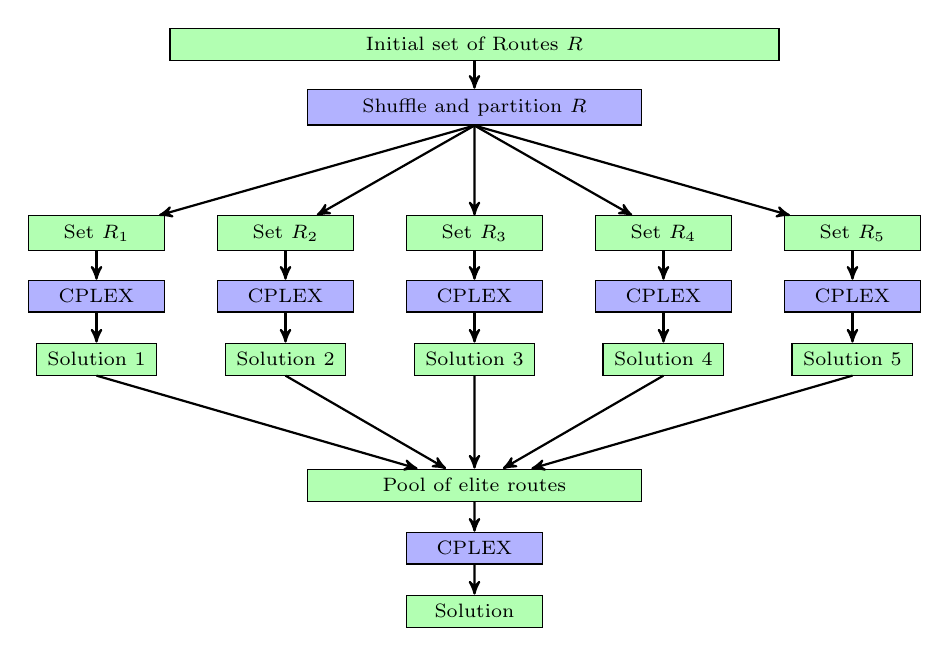
\begin{tikzpicture}[scale=0.8, auto,swap]
	
	\tikzstyle{instruct}=[rectangle, text width = 7.5cm, text  badly centered, draw]
	\tikzstyle{instruct2}=[rectangle, text width = 1.5cm, text  badly centered, draw,fill=green!30]
	\tikzstyle{instruct3}=[rectangle, text width = 1.5cm, text  badly centered, draw,fill=blue!30]
	\tikzstyle{instruct5}=[rectangle, text width = 1.3cm, text  badly centered, draw,fill=green!30]
	\tikzstyle{instruct4}=[rectangle, text width = 4cm, text  badly centered, draw]
	\tikzstyle{arc}=[->,>=stealth',thick,rounded corners=2pt, black]
	
	% placement des noeuds
	\node[instruct, fill=green!30] 	(s1) at (6,9) 	{\scriptsize{Initial set of Routes $R$}};
	\node[instruct4, fill=blue!30] 	(t1) at (6,8) 	{\scriptsize{Shuffle and partition $R$}};
	\draw[arc] (s1.south) -- (t1.north) ;
	\node[instruct2] 	(set1) at (0,6) 	{\scriptsize{Set $R_1$}};
	\node[instruct2] 	(set2) at (3,6) 	{\scriptsize{Set $R_2$}};
	\node[instruct2] 	(set3) at (6,6) 	{\scriptsize{Set $R_3$}};
	\node[instruct2] 	(set4) at (9,6) 	{\scriptsize{Set $R_4$}};
	\node[instruct2] 	(set5) at (12,6) 	{\scriptsize{Set $R_5$}};
	\draw[arc] (t1.south) -- (set1) ;
	\draw[arc] (t1.south) -- (set2) ;
	\draw[arc] (t1.south) -- (set3) ;
	\draw[arc] (t1.south) -- (set4) ;
	\draw[arc] (t1.south) -- (set5) ;
	\node[instruct3] 	(cplex1) at (0,5) 	{\scriptsize{CPLEX}};
	\node[instruct3] 	(cplex2) at (3,5) 	{\scriptsize{CPLEX}};
	\node[instruct3] 	(cplex3) at (6,5) 	{\scriptsize{CPLEX}};
	\node[instruct3] 	(cplex4) at (9,5) 	{\scriptsize{CPLEX}};
	\node[instruct3] 	(cplex5) at (12,5) {\scriptsize{CPLEX}};
	\draw[arc] (set1.south) -- (cplex1.north) ;
	\draw[arc] (set2.south) -- (cplex2.north) ;
	\draw[arc] (set3.south) -- (cplex3.north) ;
	\draw[arc] (set4.south) -- (cplex4.north) ;
	\draw[arc] (set5.south) -- (cplex5.north) ;
	\node[instruct5] 	(sol1) at (0,4) 	{\scriptsize{Solution $1$}};
	\node[instruct5] 	(sol2) at (3,4) 	{\scriptsize{Solution $2$}};
	\node[instruct5] 	(sol3) at (6,4) 	{\scriptsize{Solution $3$}};
	\node[instruct5] 	(sol4) at (9,4) 	{\scriptsize{Solution $4$}};
	\node[instruct5] 	(sol5) at (12,4) 	{\scriptsize{Solution $5$}};
	\draw[arc] (cplex1.south) -- (sol1.north) ;
	\draw[arc] (cplex2.south) -- (sol2.north) ;
	\draw[arc] (cplex3.south) -- (sol3.north) ;
	\draw[arc] (cplex4.south) -- (sol4.north) ;
	\draw[arc] (cplex5.south) -- (sol5.north) ;
	\node[instruct4, ,fill=green!30] (pool) at (6,2) 	{\scriptsize{Pool of elite routes}};
	\draw[arc] (sol1.south) -- (pool) ;
	\draw[arc] (sol2.south) -- (pool) ;
	\draw[arc] (sol3.south) -- (pool) ;
	\draw[arc] (sol4.south) -- (pool) ;
	\draw[arc] (sol5.south) -- (pool) ;
	\node[instruct3] 	(cplex) at (6,1) 	{\scriptsize{CPLEX}};
	\draw[arc] (pool.south) -- (cplex) ;
	\node[instruct2]		(end)	at (6,0) {\scriptsize{Solution}};
	\draw[arc] (cplex.south) -- (end) ;
	
	\end{tikzpicture}
	\caption{Simplified scheme of the sampling heuristics}
	\label{fig:algo1}
\end{figure}



\subsection{Refinements of the algorithm} 

Figure \ref{fig:algo1} presents an idealistic situation in which 
(i) each set $R_i, i \in 1\dots, \alpha$ yields a feasible instances that can be solved to optimality in reasonable computing time
(ii) the pool of elite routes also yields a feasible instance which is also tractable with an MILP solver. 

This is not always the case in practice. In this section, we explain how to improve the algorithm in order to avoid infeasibility and manage the size of subsets $R_i$ as well as the elite pool. 


Algorithm \ref{mainalgo} gives a more detailed description of our approach. 


In lines 12-16, sets $R_1$--$R_\alpha$ can be repeatedly used to yield elite routes. If $I_{max}=1$ the situation is like that presented by Figure \ref{fig:algo1}. Otherwise, the routes belonging to the solutions found by the MILP solver are removed from subsets $R_1 -- R_\alpha $ are the MILP solver is called again from this restricted set. This procedure can be used to extend the number of elite routes. 




\begin{algorithm}
	\caption{The sampling matheuristic}
	\label{mainalgo}
	%\scriptsize
	\begin{algorithmic}[1]
		\REQUIRE  The set $R$ of all routes generated
		\REQUIRE A parameter $\alpha$ (number of subsets)
		\REQUIRE $t1, t2$: CPU allocated to Cplex
		\REQUIRE $I_{max}$ : parameter
		\STATE $z^*= +\infty$
		\STATE $eliteRoutes \leftarrow \emptyset$
		\REPEAT
			\STATE $amelioration = FALSE$
			\STATE $R =  R \backslash eliteRoutes$
			\STATE Shuffle all routes in $R$
			\STATE $LocationSampling(R,\alpha)$ \COMMENT{partitions $R$ into at most $\alpha$ subset of routes, regrouped by starting depots}
			\STATE $RouteSampling(R,\alpha)$	\COMMENT{partition $R$ into $\alpha$ independent subsets of routes}
			\FOR{$s=1$ to $\alpha$}
				\STATE $R_s = $ routes in subset $s$
				\STATE $bestRoutes_s = \emptyset$
				\FOR {$i=1$ to $I_{max}$}
					\STATE $(z,bestRoutes_s) = solveLIRP(R_s,t1)$ 
					\STATE $eliteRoutes \leftarrow bestRoutes_s$
					\STATE $R_s \leftarrow R_s \backslash bestRoutes_s$
					
				\ENDFOR
			\ENDFOR
			\STATE 	$(z,bestRoutes) = solveLIRP(eliteRoute, t2)$
			\IF {$z < z^*$}
				\STATE $z^*=z$
				\STATE $amelioration =TRUE$
			\ENDIF
		\UNTIL {$amelioration = FALSE$}
		\RETURN $bestRoutes$
	\end{algorithmic}
\end{algorithm}






%\node[test] 	(t4) at (6,7) 	{ };
%\node[com2] 	(c4) at (t4) 		{\scriptsize{Size of pool big enough?}};
%\draw[arc] (pool.south) -- (t4.north) ;
%\node[instruct3] 	(cplex) at (6,5) 	{\scriptsize{CPLEX}};
%\draw[arc] (t4.south) -- (cplex) node[midway]{\scriptsize{yes}};
%\node[instruct2] 	(R) at (12,7) 	{\scriptsize{$R \leftarrow R \backslash R^*$}};
%\draw[arc] (t4.east) --  (R.west) node[midway]{\scriptsize{no}};


\subsection{Location based sampling}

Sampling is performed in two steps.
First, the clients are pre-assigned to a number of DCs, as described in Algorithm \ref{algo:pre-allocation}.
Then, this pre-assignment is used to build location-based subsets of routes, as described in Algorithm \ref{algo:location-sampling}.

\subsubsection{Pre-allocation of clients to depots}

One important issue in supply chain network design is the allocation of customer to DCs. 
Constraint ~\eqref{const:singleroutecustomers} states that customers are delivered by at most one route everyday. However, we don't consider single-sourcing constraints. Thus, customer can be allocated to multiple DCs. 

Algorithm \ref{algo:pre-allocation} is used to pre-allocate clients to a subset of DCs (at least one in order to ensure feasibility). 
This pre-allocation step returns a $|C| \times |D|$ matrix that defines a list of possible allocations for each client. 
This matrix will be later modified in Algorithm \ref{algo:location-sampling} when open DCs are selected. 

First, each client is pre-allocated to its closest depot (line 4). 
Then, each client is allocated to its $N_{close}$ nearest depots provided the distance between the client and the depot is not larger than a value $\mu_1$ (line 5-8).

\begin{figure}[htbp]
	\centering
	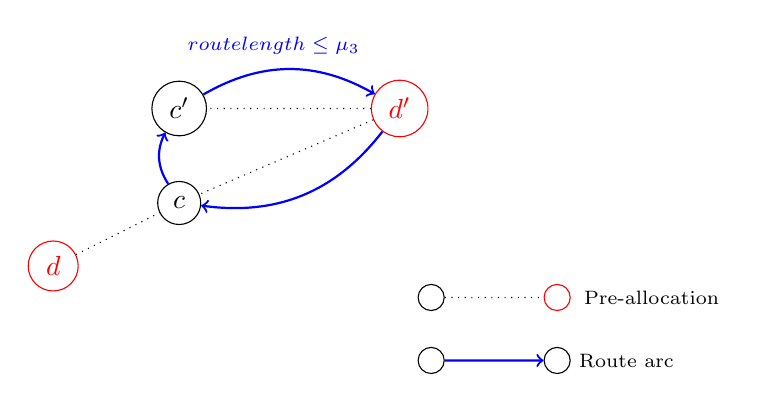
\begin{tikzpicture}[scale=0.8, auto,swap]
	
	\tikzstyle{client}=[circle,  text  badly centered, draw, color=black]
	\tikzstyle{depot}=[circle, text  badly centered, draw, color=red]
	\tikzstyle{value}=[color=blue]
	
	\tikzstyle{arc}=[->,thick, blue]
	\tikzstyle{arc2}=[dotted, black]
	
	% placement des noeuds
	\node[client] (c1) at (5,5) {$c$};
	\node[client] (c2) at (5,6.5) {$c'$};
	\node[depot] (d1) at (3,4) {$d$};
	\node[depot] (d2) at (8.5,6.5) {$d'$};
	
	\draw[arc2] (d1) -- (c1) ;
	\draw[arc2] (d2) -- (c1) ;
	\draw[arc2] (d2) -- (c2) ;
	\draw[arc] (c2) to [ bend left]   (d2)  ;
	\draw[arc] (c1) to [ bend left] (c2) ;
	\draw[arc] (d2) to [ bend left]  (c1) ;
	\node[value] (mu3) at (6.5,7.5) {\scriptsize $route length \leq \mu_3$};
	
	\node[client] (o) at (9,3.5) {};	
	\node[depot] (d) at (11,3.5) {};
	\draw[arc2] (o) -- (d);
	\node[] () at (12.5	,3.5) {\scriptsize Pre-allocation};
	\node[client] (o') at (9,2.5) {};	
	\node[client] (d') at (11,2.5) {};
	\draw[arc] (o') -- (d');
	\node[] () at (12.1,2.5) {\scriptsize Route arc};
	
	
	\end{tikzpicture}
	\caption{Pre-allocation in clusters}
	\label{fig:prealloc}
\end{figure}

Finally, lines 11--22 implement a pre-allocation rule that is specific to clusters of clients. 
As represented in Figure \ref{fig:prealloc}, 
if two clients $c$ and $c'$ are distant of no more than a value $\mu_2$, and there exists a DC $d'$ such that
$c'$ is pre-allocated to $d'$ and $dist(d',c') + dist(c',c) + dist(c,d') < \mu_3$, then $c$ is also pre-allocated to $d'$. 

 
 \begin{algorithm}
	\caption{Pre-allocations of clients to depots}
	\label{algo:pre-allocation}
	%\scriptsize
	\begin{algorithmic}[1]
		\REQUIRE  $D$: set of depots, $C$: set of clients, $N_{close}, \mu_1, \mu_2, \mu_3$: parameters, 
		$dist$: $|C|\times (|D|+|C|)$ distance matrix between clients and other clients + depot
		\STATE Initialization: $A$: $|C| \times |D|$ pre-allocation matrix filled with zeros
		\FOR {all clients $c \in C$}
			\STATE $ClosestDepots(c) = $ List of all depots $d \in D$ ranked in non-decreasing order of the distances $dist(c,d)$.
			\STATE 	$A(c,ClosestDepots(c)[1]) =1$ 	
			\FOR {$n=2$ to $N_{close}$}
				\IF {$dist(c,ClosestDepots(c)[n]) < \mu_1$}
					\STATE 	$A(c,ClosestDepots(c)[n]) =1$ 			
				\ENDIF
			\ENDFOR
		\ENDFOR
		\FOR {all clients $c \in C$ }
			\STATE Rank all clients $c' \in C$, $c' \neq c$ in non-decreasing order of the distances $dist(c,c')$ 
			\FOR {all clients $c'$}
				\IF {$dist(c,c') < \mu_2$} 
					\FOR {all $d \in ClosestDepots(c')$ such that $A(c',d)=1$}
						\IF {$A(c,d)=0$ and $dist(d,c')+dist(c',c)+dist(c,d) < \mu_3$}
							\STATE $A(c,d) =1$
						\ENDIF
					\ENDFOR
				\ENDIF
			\ENDFOR
		\ENDFOR
		\RETURN $A$
	\end{algorithmic}
\end{algorithm}






%------------------------------------------------------------
\newpage

\subsubsection{Heuristic selection of depots}

Algorithm \ref{algo:location-sampling} describes the selection of depots based on the pre-allocation of clients to depots defined by Algorithm \ref{algo:pre-allocation}. 

\begin{algorithm}
	\caption{Heuristic selection of depots}
	\label{algo:location-sampling}
	%\scriptsize
	\begin{algorithmic}[1]
		\REQUIRE $D$: set of depots, $C$: set of clients, $A$: pre-allocation matrix, $p$: number of depots to be selected, $\beta$: parameter strictly greater than 1.
		\STATE  $A' \leftarrow$  $|C| \times |D|$ allocation matrix filled with zeros
		\STATE $S \leftarrow \emptyset$: list of selected depots
		\STATE $n \leftarrow 0$: number of clients assigned to some depot
		\WHILE {$|S| < p$ and $n < |C|$ } 
			\STATE $ D \leftarrow D \backslash S$
			\STATE Rank the set of depots $D$ by non-increasing order of the number of clients assigned to each depot
			\STATE Choose a random number $y$ in interval $[0,1)$]
			\STATE $d \leftarrow$ depot at position $\lceil y^\beta \; |D| \; \rceil$ in $D$.
			\FOR {all clients $c \in C$}
				\IF {$A[c][d] =1$}
					\STATE $A'[c][d] = 1$
					\STATE $n \leftarrow n+1$
					\FOR {all depots $d' \neq d$}
						\STATE $A[c][d'] = 0$ 
					\ENDFOR
				\ENDIF		
			\ENDFOR
		\ENDWHILE
		\IF {$n < |C|$}
			\STATE Add a dummy depot $\delta$
			\FOR {all $c\in C$ such that $\sum\limits_{d \in D} A[c][d] >0$}
				\STATE $A'[c][\delta]=1$
			\ENDFOR
		\ENDIF
		\RETURN $S$ and $A'$
	\end{algorithmic}
\end{algorithm}

All non selected depots are ranked by non-increasing number of clients pre-allocated to them (line 6).
Then, a depot randomly is selected using a biased roulette wheel selection mechanism giving a much higher probability to the first depots (lines 7--8). 
Since Algorithm \ref{algo:location-sampling} is called repeatedly in Algorithm \ref{mainalgo}, this randomized selection favours diversification. 

After selecting a depot, all clients that were pre-allocated to this depot are now allocated to it (lines 10--11) 
and their pre-allocation to all other depots is cancelled (line 14). 
The final loop (lines 19--24) is used to allocate remaining clients to a dummy depot. 

\textcolor{red}{Olivier: Là je ne suis plus très sûr. Pourquoi est-ce important d'allouer les clients restant à un dépot ? Que fait-on si on n'a pas sélectionné $p$ dépots ? Et d'ailleurs comment la valeur de $p$ est elle choisie ? }

\textcolor{red}{Olivier: Question: can we have a selected DC with no customer allocated to it? If yes, remove these DCs}


\newpage

\subsection{Filtering SD routes after depot selection}

After selecting a subset of DCs and allocating clients to selected DCs, routes must be filtered in order to remove useless ones. 
In the first layer, all routes that contain at least one unselected DC are removed from the route set. 
In the second layer, routes that start at unselected DCs are removed from the route set, as well as routes visiting clients that are not allocating to the starting DC. 


%
%\begin{algorithm}
%	\caption{SD Routes filtering}
%	\label{algo:filteringSD}
%	%\scriptsize
%	\begin{algorithmic}[1]
%		\REQUIRE $SDloop$: set of SD routes
%		\REQUIRE $D$ set of depots
%		\REQUIRE $C$: set of clients
%		\REQUIRE $A$: allocation matrix
%		
%		\STATE $filteredSD \leftarrow \emptyset$
%		
%		\FOR {all $d\in D$}
%			\FOR {all $c \in C$}
%				\IF {$A[c][d]=1$}
%					\STATE $filteredSD = filteredSD \cup \{s,d\}$
%					\STATE $c = nbclient$
%				\ENDIF
%			\ENDFOR
%		\ENDFOR
%		\RETURN $filteredSD$
%	\end{algorithmic}
%\end{algorithm}
%
%
%
%\subsection{Filtering DC routes after depot selection}
%
%\begin{algorithm}
%	\caption{DC Routes filtering}
%	\label{algo:filteringDC}
%	%\scriptsize
%	\begin{algorithmic}[1]
%		\REQUIRE $DCloop$: set of DC routes
%		\REQUIRE $A$: allocation matrix
%		\REQUIRE $C$: set of clients
%		\REQUIRE $D$ set of depots
%		
%		\STATE $filteredDC \leftarrow \emptyset$
%				
%		\FOR {each route $r \in DCloop$}
%			\STATE $keep = 1$
%			\FOR {all $c \in r$}	
%				\IF{$A[c][depot(r)]=0$}
%					\STATE $keep=0$
%					\STATE $c \leftarrow $ end of the route
%				\ENDIF
%			\ENDFOR  
%			\IF {$keep=1$} 
%				\STATE $filteredDC =filteredDC \cup \{r \}$
%			\ENDIF
%		\ENDFOR
%		\RETURN $filtered DC$
%	\end{algorithmic}
%\end{algorithm}



%\begin{algorithm}
%	\caption{Generation of location oriented subsets (old version)}
%	\label{algo:location-sampling2}
%	%\scriptsize
%	\begin{algorithmic}[1]
%		\REQUIRE  $D$: set of depots
%		\REQUIRE $\alpha$: number of subsets to be generated
%		\REQUIRE $A$: pre-allocation matrix
%		\REQUIRE $\alpha$: number of subsets
%		\IF {$\alpha \ge |D|$ } 
%		\STATE $ListOfSubsets = \emptyset$
%		\STATE
%		\FOR {depot index $d=1$ to $|D|$} 
%			\STATE $ListOfSubsets = ListOfSubsets \cup \{d\}$
%		\ENDFOR
%		\STATE $NbSubsets \leftarrow |D| $		
%		\STATE
%		\STATE $n \leftarrow 2$
%		\WHILE{$NbSubsets < \alpha$}
%			\STATE $S_n$ = set of all sets of $n$ depots, ranked in non-increasing order of the number of common pre-allocated clients.
%			\REPEAT 
%				\STATE $s =$ first element of $S_n$
%				\STATE $ListOfSubsets = ListOfSubsets \cup \{s\}$
%				\STATE Remove $s$ from $S_n$
%				\STATE $NbSubsets \leftarrow NbSubsets+1$
%			\UNTIL ($S_n = \emptyset$ or $NbSubsets = \alpha$)
%		\STATE 	$n \leftarrow n+1$
%		\ENDWHILE
%		\ENDIF
%		\STATE 
%		\IF {$\alpha <  |D|$}
%			\FOR {all pairs $(i,j)$ of depots} 
%			\STATE Compute the similarity measure $M(i,j)$ equal to the number of clients pre-allocated both to $i$ and $j$.
%			\ENDFOR
%			\STATE Run $|D| - \alpha - 1$ iterations of Kruskal's algorithm with weights $\max\limits_{i,j} M(i,j) - M(i,j)$
%			\STATE $ListOfSubsets$ = one subset for each subtree yielded by Kruskal's algorithm 
%		\ENDIF
%		\RETURN $ListOfSubsets$
%	\end{algorithmic}
%\end{algorithm}


%--------------------------
\section{Numerical experiments}
\label{sec:expe}

\subsection{Constraints}

 \cite{Zheng2019} restrict the number of variables by incorporating real-life constraints that are not part of their mathematical model: 
 vehicles can visit at most four retailers at one trip due to vehicle capacity limitation, and DCs can only serve retailers within a given radius. 
 These constraints help reduce the number of variables from 3 millions to 600 thousands.
 


\section{Conclusion}


\subsection*{Possible extensions}
\begin{itemize}
	\item Etendre au cas où le coût d'une route dépend de sa charge.
\end{itemize}


\end{linenumbers}

\newpage
\bibliographystyle{abbrvnat}
\bibliographystyle{plain}
\bibliography{biblio_LIRP}

\end{document}
